\chapter{Results} 
\label{chap:results}
%\begin{enumerate}
%\item all data
%\item analysis done
%\item discussions
%\item comparisons
%\end{enumerate}

\begin{figure}
  \begin{center}
    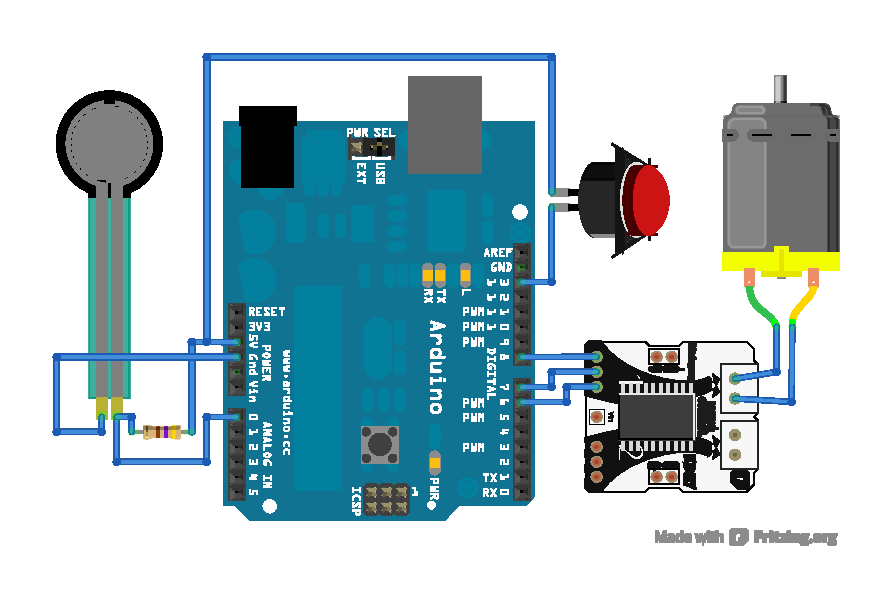
\includegraphics[width=1.0\columnwidth]{Figures/simple-example.pdf}
    \caption{The components of a simple single-board \xten setup} \label{fig:singleboard}
  \end{center}
\end{figure}

This chapter presents evidence showing how the \xten architecture achieves its objectives through the hardware and software platform. We demonstrate this by applying the framework across a number of practical examples before discussing the outcomes.

 We demonstrate the framework in action by showing excerpts of sample programs for a simple mobile robot with a number of sensors and actuators distributed across one or more daughterboards. These examples demonstrate how modularity, scalability and extensibility are expressed through code and hardware configuration.
 
All tests and examples were done using the Arduino Prototyping system since this was the chosen platform used to prototype the \xten architecture. The fundamental concepts however were general enough to be implemented on any modern microcontroller.

Listing~\textbf{\ref{code:example}} is a typical code setup for a very simple mobile robot illustrated in Figure \textbf{\ref{fig:singleboard}}. All the sensors and actuators were placed on one board; for this particular implementation, we utilised the \textbf{internal} daughterboard which is hosted on the same board as the motherboard. This robot has one actuator (a DC motor connected to an external H-bridge), a force sensor and a pushbutton sensor.


%\begin{multicols}{2}
	\begin{listing}
		\footnotesize
		\begin{minted}[bgcolor=bg,baselinestretch=1,frame=lines,framesep=2mm,label={\xten Sample code}]{c}

/**
* Import the necessary libraries for the motherboard, 
* internal daughterboard and the peripheral bus
**/
#include <Wire.h>  
#include <X10ABOT_MB.h>
#include <X10ABOT_DB.h> //Include the internal daughterboard #0 (SELF)

//Initialise the DC motor on daughterboard #0 (SELF), actuator port #1
Actuator motor1(SELF,1);
//Initialise force sensor on daughterboard #0 (SELF), sensor port #1
Sensor force1(SELF,1);
//Initialise force sensor on daughterboard #0 (SELF), sensor port #2
Sensor pushbutton(SELF,1);

void setup(){}
void loop(){
//Continuously check the sensors for a reading
  if(pushbutton.readDigitalB() || (force1.readAnalog()>100)){
    motor1.aB(); //Turn motor1 on by sending LO on pin a and HI on pin B
    motor1.pwm_a(100); //operate motor1 at full power (100%) 
  }else{
    motor1.ab();//Turn motor1 off by sending LO on pin a and pin b
  }
}	 
	\end{minted}
		\caption{Example of the \xten architecture on a simple - single board robot.} \label{code:example}
	\end{listing}
%	\vfill
%	\columnbreak



Listing~\textbf{\ref{code:example}} is a simple program that drives the motor at full speed if either the touch sensor records an input or if there is a force on the force sensor above a certain threshold, otherwise the motor will be given the off signal.

%\end{multicols}
In this instance, there are two types of devices that are declared, \textbf{Sensor} and \textbf{Actuator}. These represent the parent classes of all sensors and actuators respectively in the \xten architecture. This example utilises the parent class but for more complex sensors and actuators, a subclass would have been appropriate. All other sensor and actuator sub-types inherit from these two classes of devices, overriding where necessary.

It should be noted that it was necessary to include the library for both the motherboard and the daughterboard since they share the same Arduino board. Daughterboard address \#0 or the constant \textbf{SELF} is reserved for the internal daughterboard on the same physical Arduino platform.

	\section{Modularity} % (fold)
	\label{sec:modularity}
% section modularity (end)
Adding an extra capability was easily and seamlessly carried out using the \xten architecture. We included an extra daughterboard that represented a complete subsystem using sensors and actuators. In our example in Figure \textbf{\ref{fig:modularity}}, an extra DC motor and a light sensor were added as a single module. The \xten architecture allowed for this new addition as a daughterboard via the peripheral bus. The module was just as easily added in software. The daughterboard was assigned a unique arbitrary address of \textbf{\#9}. Instructions were then added to activate the new DC motor if there was light intensity above a certain threshold on the sensor. We could have easily controlled the existing motor or mixed the logic between the existing components, however for clarity we made it so that the modules would operate independently.  In the Listing~\ref{code:modularity}, we demonstrate how we added this extra functionality.

\begin{figure}[h!]
  \begin{center}
    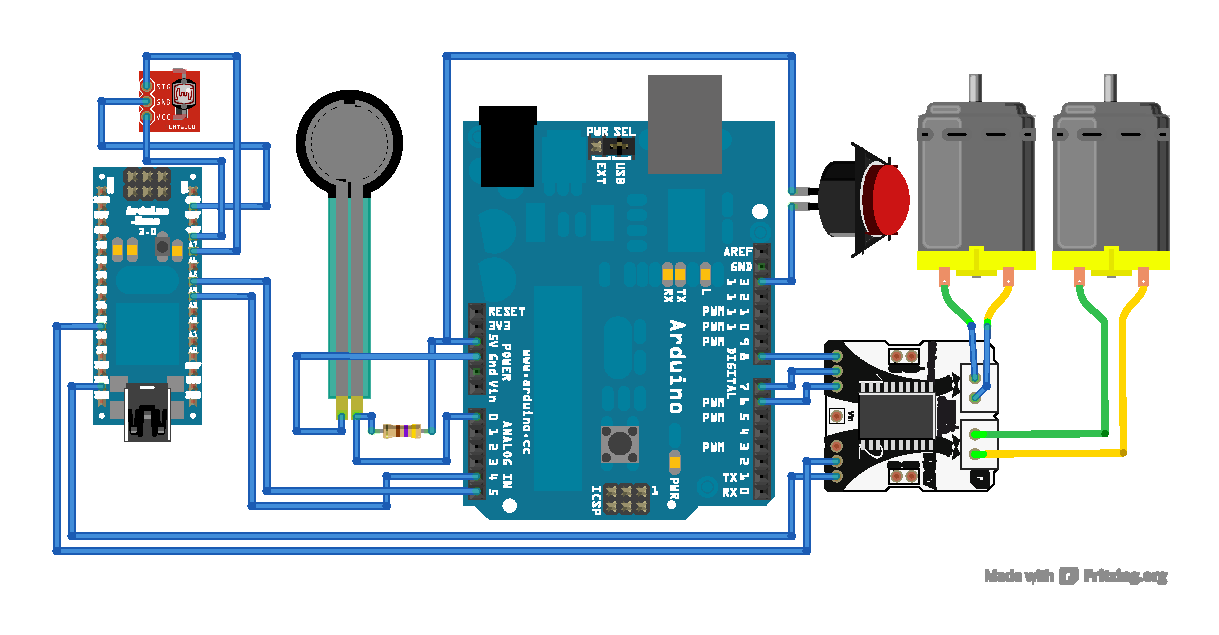
\includegraphics[width=1.0\columnwidth]{Figures/modular-example.pdf}
    \caption{The components of a Modular single-board \xten Example}\label{fig:modularity}
  \end{center}
\end{figure}

\begin{listing}
		\footnotesize
        {\fontsize{8}{6}\selectfont
		\caption{Example of code modularity (the code components were separated to emphasise modularity). Highlighted region indicates the code added for the new module} \label{code:modularity}
		\begin{minted}[bgcolor=bg,baselinestretch=1,frame=lines,framesep=2mm,label={Modularity in Code}]{c}
        \end{minted}
        \begin{minted}[bgcolor=bg,baselinestretch=1]{c}
/**
* Import the necessary libraries for the motherboard, 
* internal daughterboard and the peripheral bus
**/
#include <Wire.h>  
#include <X10ABOT_MB.h>
#include <X10ABOT_DB.h> //Include the internal daughterboard #0 (SELF)

//Initialise the DC motor on daughterboard #0 (SELF), actuator port #1
Actuator motor1(SELF,1);
//Initialise force sensor on daughterboard #0 (SELF), sensor port #1
Sensor force1(SELF,1);
//Initialise force sensor on daughterboard #0 (SELF), sensor port #2
Sensor pushbutton(SELF,1);
   
void setup(){}
void loop(){
//Continuously check the sensors for a reading
if(pushbutton.readDigitalB() || (force1.readAnalog()>100)){
    motor1.aB(); //Turn motor1 on by sending LO on pin a and HI on pin B
    motor1.pwm_a(100); //operate motor1 at full power (100%) 
  }else{
    motor1.ab();//Turn motor1 off by sending LO on pin a and pin b
  }
 \end{minted}
 \begin{minted}[bgcolor=hilite,baselinestretch=1]{c}
 const byte BOARD2 = 9; //Constant with arbitrary daughterboard address
 //Declare motor on daughterboard #9, actuator port #1
 Actuator motor2(BOARD2,1);
 //Declare force sensor on daughterboard #9, sensor port #1
 Sensor lightSensor(BOARD2,1);
 
//Added extra functionality with a new sensor and a new actuator
//on daughterboard #9 while light is on the sensor, activate motor2
if (lightSensor.readAnalog()>700)
  {
    motor2.Ab(); //Turn motor2 on by sending HI on pin A and LO on pin b
    motor2.pwm_a(50); //operate motor2 at half power (50%)
  }else{
    motor2.ab();//Turn motor1 off by sending LO on pin a and pin b
  }
}	 
	\end{minted}
		}
\end{listing}
In the code example at Listing \textbf{\ref{code:modularity}}, even with the addition of two independent devices, \emph{motor1} and \emph{lightSensor} to the system, that did not affect the existing code but fit seamlessly in the development process. Separate code was added to carry out their operation which never needed to interact with the existing system. There needed to be no special accommodation for the new module in the existing code. There was no significant modification made to the existing hardware setup even with the fact that an extra physical component, another daughterboard, was added to the system. The \xten design allowed a pluggable interface that facilitated adding new code and hardware with minimal modification to the existing setup.
All these features are an indication of a truly modular architecture. As previously defined, we included an entire subsystem without modifying the existing components. The modules can be removed just as easy as they were installed. The level of expertise, with regard to specialised knowledge required to modify this system is also relatively minimal when compared to a generic prototyping platform like the Arduino due to the abstraction in its design.


% chapter findings_and_results (end)
\section{Extensibility and Abstraction} % (fold)
\label{sec:extensibility_abstraction}
We demonstrate the \xten architecture's ability to support new and varied types of sensors and actuators. This is accomplished by creating a subclass to either of the existing Sensor or Actuator classes. These parent classes support all the generic operations on all the available sensor and actuator ports. By creating a subclass, all the parent class properties and functions will be inherited. Devices with unique configurations can be supported by utilising the same abstracted daughterboard access available to the parent classes requiring no knowledge of the low-level details of the hardware.
In the following example, we will define a simple, yet complete library that reads and interprets the data from a thermistor temperature sensor. The raw analog value will be read then we will apply some computations to acquire a useful output. The class will support functions that return temperature values in both celsius and fahrenheit units. This code was originally sourced from the Arduino Playground~\parencite{therm} as a simple example to acquire thermistor temperature readings. We made a few simple modification that allowed the same code to be applicable to the \xten architecture.
\begin{listing}
		\footnotesize
        {\fontsize{8}{6}\selectfont
		\caption{Example: A complete library for a thermistor temperature sensor. The highlighted region indicates where the \xten microcode was added.} \label{code:therm}
		\begin{minted}[bgcolor=bg,baselinestretch=1,frame=lines,framesep=2mm,label={Thermistor Library}]{c}
#include "../X10ABOT_MB.h"
#include <math.h>
class Thermistor: public Sensor
{
  private:
    byte _db, _port;
  public:
    Thermistor(byte db_address, byte port_number):Sensor(_db, _port){
      _db = db_address;
      _port = port_number;
    }
    ~Thermistor(){};
    double readThermistorCelsius() {
    \end{minted}
    \begin{minted}[bgcolor=hilite,baselinestretch=1]{c}
        //The analog microcode requests the raw sensor value
        int RawADC = analog(_db,_port); 
    \end{minted}
    \begin{minted}[bgcolor=bg,baselinestretch=1]{c}
        double Temp;
        Temp = log(((10240000/RawADC) - 10000));
        Temp = 1/(0.001129148+(0.000234125+(0.0000000876741*Temp*Temp))*Temp);
        Temp = Temp - 273.15;            // Convert Kelvin to Celsius
        return Temp;
    }
    double readThermistorFarenheit() {
    // Convert Celsius to Fahrenheit
        return (readThermistorCelsius()* 9.0)/ 5.0 + 32.0;
    }
};
	\end{minted}
		}
\end{listing}

The conversion instructions of the \xten library in Listing \textbf{\ref{code:therm} }is an almost exact replica of the fragment of code extracted from the Arduino Thermistor library. In the \textbf{readThermistorCelsius} function, the main change (highlighted in yellow) can be found where the code accesses the analogue pin to read the raw data value acquired from the sensor. These functions are at the the lowest level of abstraction and are used to read and write to the individual pins of each port. They include \emph{digitalIn, digitalOut, pwm and analog.} For this particular case, the \textbf{analog(\_db,\_port)} microcode function was invoked, access to this function was inherited by extending the Sensor class. This is a method used to abstract sensor port's analog pin so that it becomes hardware independent. The sensor port (\textbf{\_port}) belongs on a daughterboard (\textbf{\_db})where it accesses the data from the  analogue pin. The raw analogue value is then returned to the calling function where it is further processed.

This thermistor library can then be easily utilised by the user as follows (See Listing \ref{code:thermcode}):

The code in Listing~\textbf{\ref{code:thermcode}} presents a temperature monitoring system that watches the temperature that it receives from two thermistors. If the value read from the thermistors goes beyond particular thresholds for either of them, an alarm is triggered.
\begin{listing}
		\footnotesize
        {\fontsize{8}{6}\selectfont
		\caption{Example application of the thermistor temperature sensor library.} \label{code:thermcode}
		\begin{minted}[bgcolor=bg,frame=lines,baselinestretch=1,framesep=2mm,label={Thermistor Example Application}]{c}
#include <Wire.h>  
#include "x10sions/Thermistor.h"
#include <X10ABOT_MB.h>
const byte FREEZER = 17; //Create a constant with the daughterboard address
const byte OVEN = 108;
const byte CONTROL_BOARD = 10;

//Declare thermistor on daughterboard #17, sensor port #1
Thermistor coldSensor(FREEZER,1);
//Declare thermistor on daughterboard #108, sensor port #6
Thermistor hotSensor(OVEN,6);
//Declare digital alarm on daughterboard #10, actuator port #3
Actuator alarm(CONTROL_BOARD,3,A);

void setup(){}
void loop(){
//Continuously check the sensors to see if temperature within threshold
  if((coldSensor.readThermistorCelsius() > 1 )
      || hotSensor.readThermistorFarenheit()<200){
  alarm.on_a(); //Turn on alarm 
  }
}
	\end{minted}
		}
\end{listing}

A typical end user would not be involved in creating libraries for sensors. They would have only been exposed to the setup in Listing~\ref{code:thermcode}. The only requisite knowledge would be familiarity with the supported list of functions specified for a thermistor. In this case only \textbf{readThermistorFarenheit()} and  \textbf{readThermistorCelsius()} are specified and both have been used.
The library for a thermistor was included and it became very straightforward to utilise the sensor readings afterwards.
% section extensibility and abstraction (end)

\section{Scalability} % (fold)
\label{sec:scalability}

% section scalability (end)
Based on the results gathered from testing for modularity, an inherent property for scalability can be observed. The method of modular addition lends itself to be scalable to tens of modules as defined by the specifications of the \iic peripheral bus protocol. Scalability is not only measured by how many devices can be connected to the system, but we must take into consideration the performance of the system when all these devices are operational. To investigate this, we benchmarked the performance of the architecture that we implemented on the Arduino platform.  When operating with daughterboards across the peripheral bus, the \xten architecture's major limiting factor becomes the speed of data transfer. The default speed of the \iic peripheral bus when using the Arduino platform is 100Kb/s, this can be further configured to go as high as 400Kb/s. For our application on the Arduino we had best result when performing between 230Kb/s and 300Kb/s. We performed a number of tests to determine the latency of each type of basic instruction (microcode) to see how they would affect the performance of the entire system. All tests below were carried out on the Arduino Mega, using the Atmel \texttrademark ATMega1280 microcontroller.

We carried out instruction execution latency tests to evaluate the performance of the \xten framework on the Arduino platform. We performed three sets of test comparing the speed of execution on:
\begin{itemize}
\item  An Arduino without the \xten framework.
\item The \xten framework with a single daughterboard on the peripheral bus
\item The \xten framework with no external daughterboards (internal daughterboard used instead).
\end{itemize}

The tests were carried out by invoking and storing the value of Arduino\'s \textbf{micros()} function which returns the number of microseconds since the program started. The times before and after function executions were recorded and their difference taken. The timing utility on the Arduino has a maximum resolution of 4 micro second intervals therefore the readings were not precise. We implemented the tests in a continuous loop and recorded a sample of 20 consecutive duration time values for each tested function. We did further computations to find the mean and the standard deviation (Figure~\ref{eq:sd}) of the sample set of these values.

$$
s = \sqrt{\frac{1}{N-1} \sum_{i=1}^N (x_i - \overline{x})^2}
$$
\captionof{figure}{The Sample Standard Deviation equation}\label{eq:sd}

\newpage
\textbf{The tables below display the result of our timing experiment: }

\begin{table}[h!]
	\caption{Table showing instruction latency in microseconds($\mu$s) for a regular Arduino using a sample of 20 consecutive executions.}\label{table:arduinoboard}
	\begin{tabular}{|l|l|l|l|l|}
	\toprule
 \multicolumn{5}{c}{\textbf{Direct Arduino Board readings}} \\\hline

& digitalOut & digitalIn & pwm & analogue \\\hline
Mean:                   & 13.6 & 15.6 & 12.2 & 115.6\\\hline
Standard Deviation:     & 2.01 & 2.21  & 0.89  & 3.41 \\\hline
3 Stnd. Devs. Lower Limit& 7.57 & 8.97  & 9.53  & 105.37 \\\hline
3 Stnd. Devs. Upper Limit& 19.63& 22.23 & 14.87 & 125.83 \\\hline
\end{tabular}
\end{table}
%The Sample digitalOut: %[12, 12, 16, 16, 12, 12, 12, 16, 16, 12, 12, 16, 16, 12, 12, 12, 16, 16, 12, 12]
%average = 13.6
%s = 2.01
%The Sample digitalIn: %[20, 16, 16, 16, 16, 12, 16, 16, 12, 16, 16, 12, 16, 16, 12, 16, 16, 20, 16, 16]
%average = 15.6
%s = 2.21
%The Sample pwm: %[12, 12, 12, 12, 12, 12, 12, 12, 12, 12, 12, 12, 12, 12, 12, 12, 12, 16, 12, 12]
%average = 12.2
%s = 0.89
%The Sample analogue:%[112, 120, 116, 116, 116, 124, 112, 112, 112, 120, 116, 116, 116, 116, 112, 112, 112, 120, 116, 116]
%average = 115.6
%s = 3.41

\begin{table}[!ht]
	\caption{Table showing microcode instruction latency in microseconds($\mu$s) for the the on-board daughterboard using a sample of 20 consecutive executions.}\label{table:onboard}
	\begin{tabular}{|l|l|l|l|l|}
	\toprule
 \multicolumn{5}{c}{\textbf{One Board \xten readings}} \\\hline

& digitalOut & digitalIn & pwm & analogue \\\hline
Mean:                   & 39.4 & 83.58 & 57.8 & 215.58\\\hline
Standard Deviation:     & 2.15 & 2.27  & 4.17  & 2.95 \\\hline
3 Stnd. Devs. Lower Limit	&32.95	&76.77	&45.29	&206.73\\\hline
3 Stnd. Devs. Upper Limit	&45.85	&90.39	&70.31	&224.43\\\hline
\end{tabular}
\end{table}
%The Sample digitalOut:% [40, 40, 36, 40, 40, 40, 40, 40, 36, 40, 40, 40, 40, 40, 36, 40, 40, 40, 40, 40]
%average = 39.4
%s = 2.15
%The Sample digitalIn:% [84, 88, 84, 84, 84, 84, 84, 80, 84, 80, 88, 84, 84, 84, 80, 84, 84, 80, 84]
%average = 83.58
%s = 2.27
%The Sample pwm:% [60, 56, 56, 56, 60, 60, 56, 56, 60, 60, 56, 56, 56, 60, 60, 56, 56, 60, 60, 56]
%average = 57.8
%s = 4.17
%The Sample analogue:% [212, 216, 212, 216, 212, 212, 212, 216, 216, 216, 216, 216, 216, 216, 220, 216, 216, 224, 216215.58]
%average = 215.58
%s = 2.95

\begin{table}[!ht]
	\caption{Table showing microcode latency in microseconds($\mu$s) for a daughterboard connected over the peripheral bus using a sample of 20 consecutive executions.}\label{table:offboard}
	\begin{tabular}{|l|l|l|l|l|}
	\toprule
 \multicolumn{5}{c}{\textbf{Two Board \xten readings}} \\\hline

& digitalOut & digitalIn & pwm & analogue \\\hline
Mean:                       & 261.4 & 554.8 & 319   & 685.2\\\hline
Standard Deviation:         & 2.98  & 2.63  & 2.20  & 5.43 \\\hline
3 Stnd. Devs. Lower Limit	& 252.46	&546.91	&312.4	&668.91	\\\hline
3 Stnd. Devs. Upper Limit	& 270.34	&562.69	&325.6	&701.49	\\\hline
\end{tabular}
\end{table}

%The Sample digitalOut:% [260, 268, 260, 260, 260, 260, 260, 260, 268, 260, 264, 260, 260, 260, 260, 268, 260, 260, 260, 260]
%average = 261.4
%s = 2.98
%The Sample digitalIn:% [556, 556, 556, 552, 556, 552, 560, 556, 552, 552, 556, 552, 556, 560, 556, 552, 552, 556, 552, 556]
%average = 554.8  
%s = 2.63
%The Sample pwm :%[320, 316, 320, 320, 320, 320, 320, 316, 320, 324, 316, 320, 320, 316, 320, 316, 320, 316, 320, 320]
%average = 319
%s = 2.20
%The Sample analogue:% [668, 656, 668, 656, 656, 660, 656, 664, 656, 656, 656, 656, 652, 656, 656, 656, 656, 652, 672, 656]
%average = 658.2
%s = 5.43


\section{Observations} % (fold)
\label{sec:Observations}

From the results, we have observed that the latency for output operations took notably less time than that of input operations. This was expected since input operations consist of two instructions over the peripheral bus. The first is a request for the data and the second is a retrieval. We had to intentionally slow down the speed of the second request from 300Kb/s to 230Kb/s to allow time for the daughterboard to retrieve the requested data. We attempted faster speeds but it resulted in periodic data loss. Output operations only required that one instruction be sent across the bus.

We calculated the standard deviation and presented the data ranges for up to three standard deviations. These upper and lower limits indicate the statistical prediction of the maximum and minimum execution time for each function with about 99.7 percent confidence. The end user can then determine if this latency is acceptable for their application.

We also presented a comparative analysis of the Arduino with and without the \xten system. We observed that the all readings on all platforms fell below the 1 millisecond mark. For most school based or hobbyist projects, this falls within an acceptable range since realtime response is rarely required.

The results emphasised that the advantages of \xten platform are more pronounced when it has to manipulate devices across multiple daughterboards. There are tradeoffs in performance which had to be sacrificed to accomplish this but it allowed the the framework to achieve its goals of being modular, scalable and extensible.
% section economy (end)
